
\section{Data Analysis}

There are three scenarios included in our research, namely, the most vibrant city, the popular sports and fitness enthusiasts. 

Data utilized here are from Twitter, AURIN, and ESPN, which are stored in CouchDB. Twitter users typically post varieties of content, where texts, locations, and usernames are used here to identify patterns in three scenarios. As for data from the AURIN platform, we assume these are relevant in the context of the vibrant city (scenario 1). To recognize the fitness enthusiast (scenario 3), the tough sports ranking from ESPN is one of the key measurements.


\subsection{Scenario analysis}

\subsubsection{Overview}
AURIN data can be easily stored in CouchDB and imported after selecting features and merging results through Python. As for the sports list and difficulty ranking, we add different tense of each sport as well as its synonymous manually before they are stored in two lists or arrays in views. While for original Twitter data on CouchDB, Django application, CouchDB map reduce and Spark are utilized to obtain the result. 

For Twitter data, the CouchDB view is defined firstly to extract special data, which includes a map function written in JavaScript and a reduced function embedded in the database. Django then sends a \mintinline{python}{GET} request to draw results from the CouchDB view through CouchDB REST API. After feeding the initial result to Django, it then invokes the analyzer Python code to further process the data. Finally, the conclusion is constructed through the Django view, which can be accessed from the Django REST framework, and then can be loads to the maps, graphs, and charts, and this is illustrated in Figure \ref{couchdb and django}.

An emerging challenge during the analysis stage is that only predefined reduce functions are supported by CouchDB, such as \mintinline{python}{_count}, \mintinline{python}{_sum}, etc, which might be hard for us to gather the result for scenario 3 analysis. To address this issue, Spark application is introduced, whose details is described in scenario 3. 


\subsubsection{Scenario 1: The most vibrant city}
Key characters of being vibrant are assumed to be energetic, enthusiastic, active, healthy, and alive. Therefore, seven elements are considered when we spot the most vibrant city, including factors generated from AURIN, such as gender, median age, median income, unemployment rate, and education levels, as well as the measurements generated from Twitter (the number of sports tweets). The score of each factor is given to every six cities from 1 to 6. For example, the more unbalanced the gender distribution in a city, the more points the city will lose. If the city's educated rate ranks the least, then this city will gain 1 point in terms of this factor. While in the city's rank the highest in educated rate, 6 points will be earned by this city. 

\paragraph{CouchDB MapReduce and Django view}

One of the key measurements of a vibrant city is the number of sports tweets post by the users living in this area. Assuming the more they post sports tweets, the more they enjoy workouts and are active. To obtain the total number of sports tweets in each city, MapReduce in CouchDB is used to filter and summarize tweets including any 1 of 75 sport types by using the reduce function \mintinline{python}{_sum}. Specifically, in the map function, we use 75 emit(key, value) functions where the key is tweet ID, and the value is a set including 75 sports with one of the sport's values being 1. If the current tweet text contains any sport, an entry then is created in the view result with the value of the sport equals 1 in the value section. By using \mintinline{python}{_sum}, it sums up values of all entries according to sport type. After that, the Django view is used, to sum up, all the sports results for each city by replacing the city name (partition name) in CouchDB restful API. 

\begin{lstlisting}[language=JavaScript, caption= Map Functions for Sports Tweets, backgroundcolor = \color{white}]
function (doc) {
    var sport = /[^a-zA-Z]racing[^a-zA-Z]/;
    if (sport.test(doc.val.text.toLowerCase())){
    emit(doc._id, {`racing': 1, `gokart': 0 ,...,`diving': 0}); //75 sports elements
    
    var sport = /[^a-zA-Z]gokart[^a-zA-Z]/;
    if (sport.test(doc.val.text.toLowerCase())){
    emit(doc._id, {`racing': 0, `gokart': 1, ,...,`diving': 0});
    
    ... //the rest emit functions 
    
    var sport = /[^a-zA-Z]diving[^a-zA-Z]/;
    if (sport.test(doc.val.text.toLowerCase())){
    emit(doc._id, {`racing': 0, `gokart': 1, ...,`diving': 1});}
\end{lstlisting}

To analyze the sports trend of each city further, the number of sports tweets of each city from 2019 to 2021 is gathered. Specifically, 3 views filtering sports tweets in 2019, 2020, and 2021 should be created respectively in CouchDB first, with the reduced function \mintinline{python}{_sum}. The map function is very similar to the one mentioned above, both of them filtered sports tweets, while this map function adds one more condition. The method \mintinline{python}{date.getFullyear()} is used here to filter related yearly sports tweets. After the view result is initialized, we use Django view to invoke the analyzer code and call the restful URL, which loops 3 years for each city. Finally, the result is returned through web browsable API on the REST framework. 



\paragraph{Result}

\begin{figure}[H]
\centerline{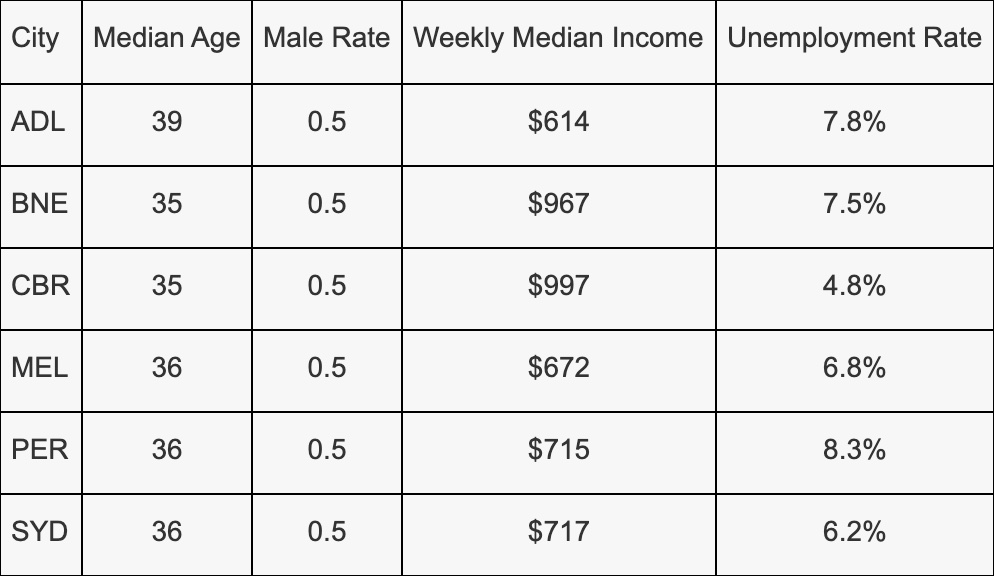
\includegraphics[width=3in]{Figures/age,income,gender.jpg}}
\caption{Age,Income, Gender and Unemployment\label{Age,Income, Gender and Unemployment}}
\end{figure}


Females and males are evenly distributed across four cities, while the median age shows a different pattern. Adelaide had the oldest median age of six capital cities at 39 years, followed by Melbourne, Sydney, and Perth at 36, while Canberra and Brisbane were the youngest, at 35. Interestingly, it is also people living in Canberra have the highest median income, nearing \$1000 per week, while the median income in every other state city ranges from \$600 to \$700 (Figure \ref{Age,Income, Gender and Unemployment}). As for employment and education, the unemployment rates across six cities are all under 9\%, with the highest number seen in Perth and Adelaide, and the lowest in Canberra, at around 5\%. Interestingly, Canberra is ranked the most educated capital city based on percentage, as well as has the highest number of people with a bachelor’s degree or higher. It is Adelaide, however, ranked least with an educated rate (Figure \ref{education}). 

\begin{figure}[H]
\centerline{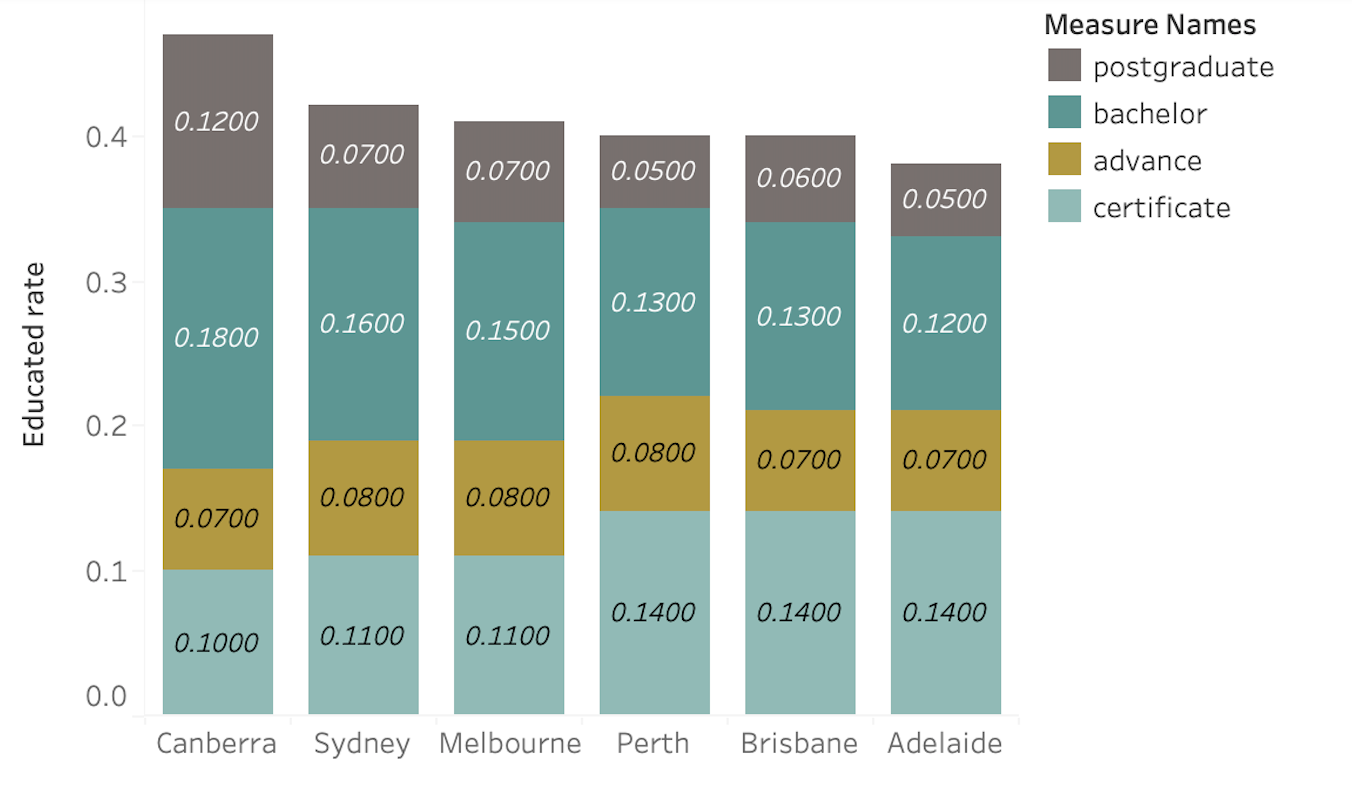
\includegraphics[width=4in]{Figures/education.png}}
\caption{Education Levels\label{education}}
\end{figure}

Regarding the sports tweets, this result is shown on the map where six circles represents for six cities and the circle size depends the number of sports tweets posted in the city (Figure \ref{map}). Adelaide posts the most sports tweets, which is followed by Melbourne and Sydney, while Perth and Brisbane post the least sports contents. By taking account of the number tweets of each area, the sports tweets ratio is used as a more objective measurement here (Figure \ref{fig:sports ratio}). Users in Adelaide still dominates in posting the sports-related content, at 2\%, which is more than twice as high as the percentage in Melbourne. It is worth pointing out that sports tweet content percent in Perth ranks the second, while users in Sydney turns out to post the least sports content. The reason of changes of ranking might be the unbalance distribution of active Twitter users in big cities and small cities. Noticeably, the rank of sports tweets among six cities has been the same for the last three years (Figure \ref{fig:sports tweets since 2019}), and a significant rise can be seen in each city. This means that Twitter users are likely to post more sport-related tweets than ever.

\begin{figure}[H]
\centerline{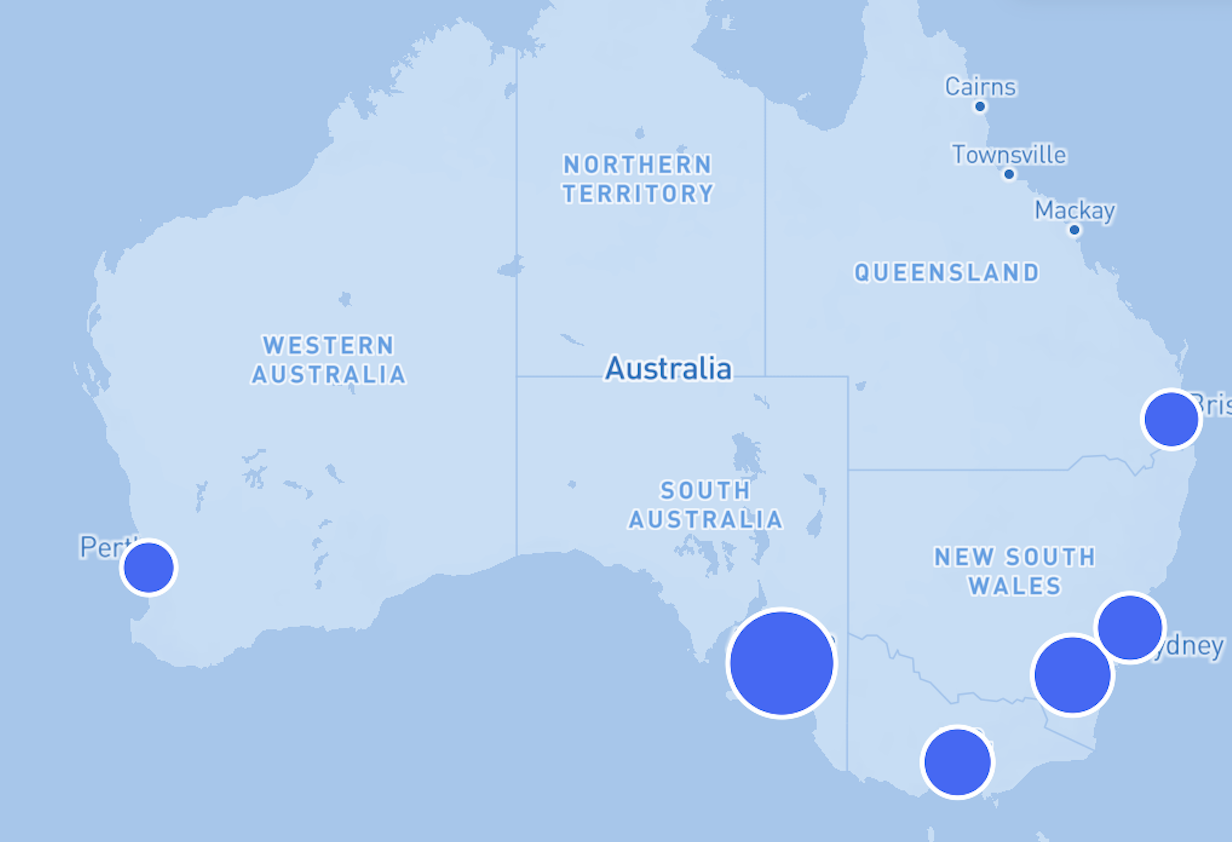
\includegraphics[width=3.5in]{Figures/Screen Shot 2021-05-25 at 8.47.44 pm.png}}
\caption{Map\label{map}}
\end{figure}

\begin{figure*}[h!]
\centering
\begin{minipage}[t]{0.48\textwidth}
\centering
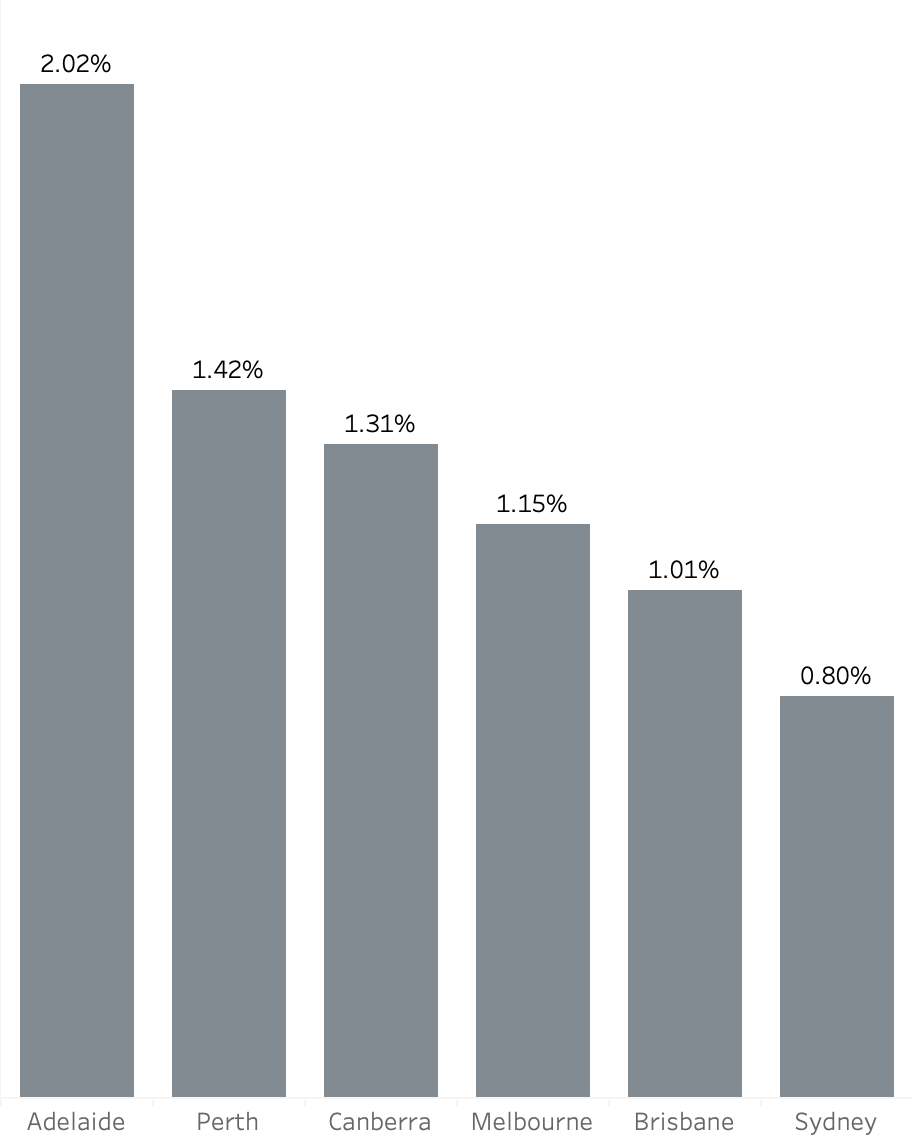
\includegraphics[width=8cm]{Figures/sports rate.png}
    \caption{Sports Tweets Ratio}
    \label{fig:sports ratio}
\end{minipage}
\begin{minipage}[t]{0.5\textwidth}
% \hspace{-2cm}
\centering
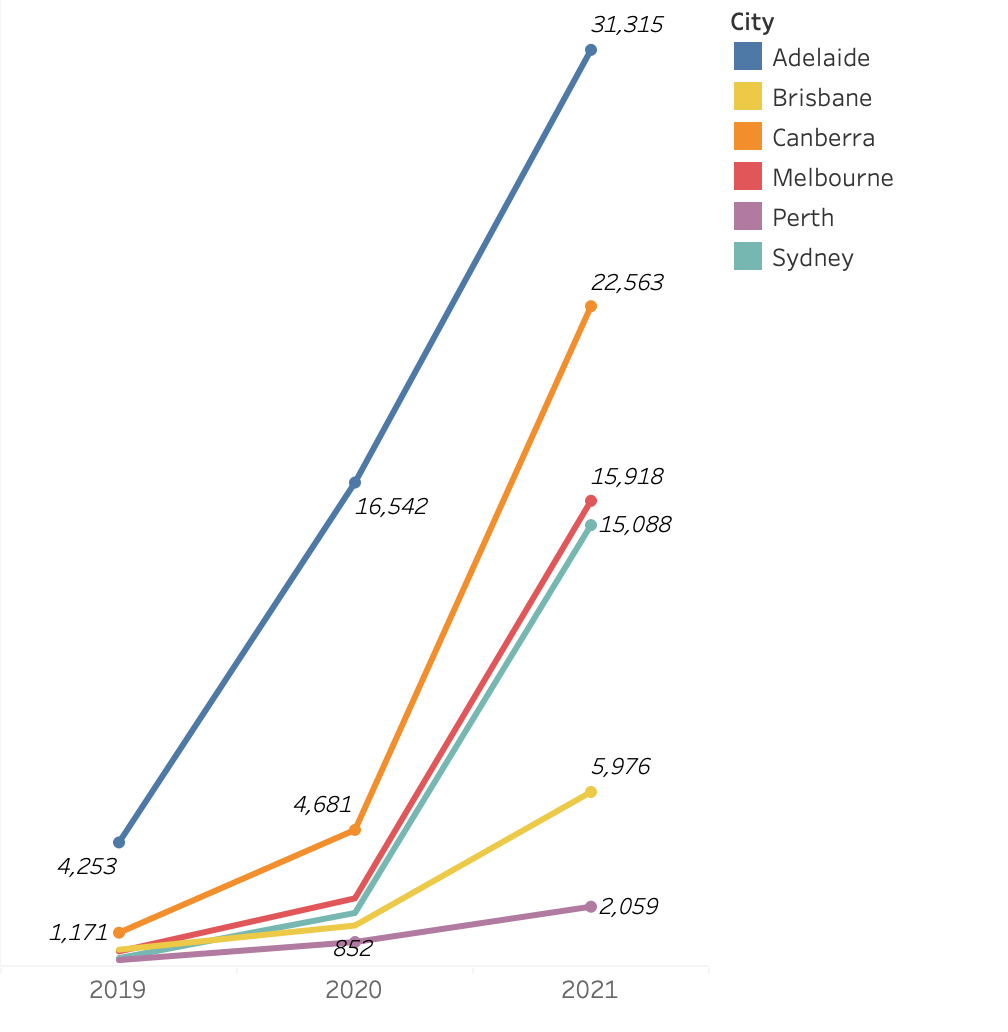
\includegraphics[width=9cm]{Figures/2019-2021.png}
    \caption{Sports Tweets since 2019}
    \label{fig:sports tweets since 2019}
\end{minipage}
\end{figure*}

\begin{figure*}[h!]
\centerline{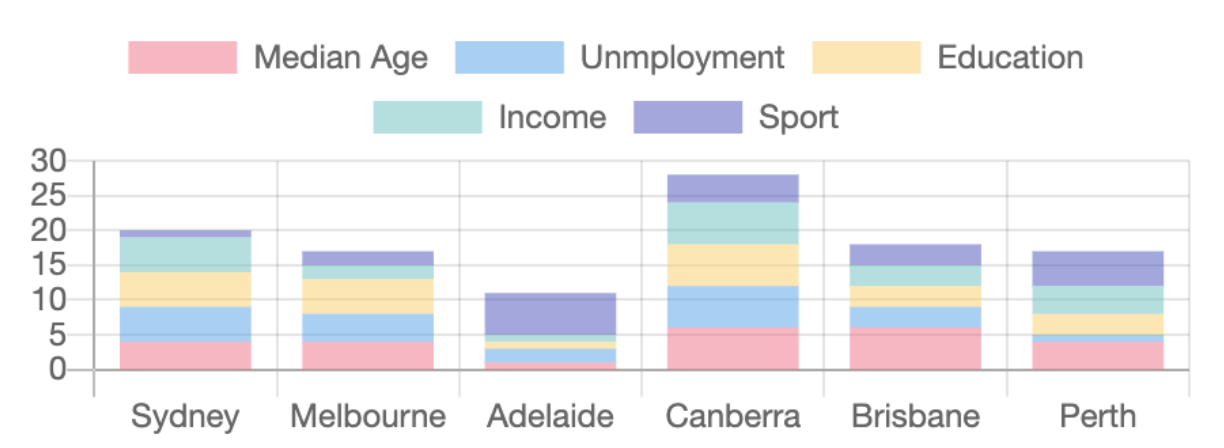
\includegraphics[width=4in]{Figures/vibrant city.png}}
\caption{The Vibrant Cities\label{vibrant result}}
\end{figure*}

According to the 6 factors (gender, age, income, unemployment, education, and sports tweets) discussed above, Canberra wins the most vibrant city (Figure \ref{vibrant result}), as it has earned the most points. This is followed by Sydney and Melbourne, while Adelaide ranked the least in this part.

\subsubsection{Scenario 2: Popular sports}
Assuming the higher the number of sport-related tweets is, the more popular the sport is. During this sports analysis, Twitter data is used to identify the most popular sports across Australia as well as each city respectively. 

\paragraph{CouchDB MapReduce and Django view}
This map function of the CouchDB view is the same one as we showed above. 75 \mintinline{python}{emit ()} functions are used to create entries for each type of sports tweet, and only the mentioned sport in the tweet returns 1. Then the reduce function \mintinline{python}{_sum} is used to summarize the total number for each sport. However, in the Django view, we do not need to sum up all sports results for each city. Instead, the Django REST framework returns each sports popularity result for each city, as well as for all cities. This can be done by writing Python in Django view.

\paragraph{result}
\begin{figure*}[h!]
\centerline{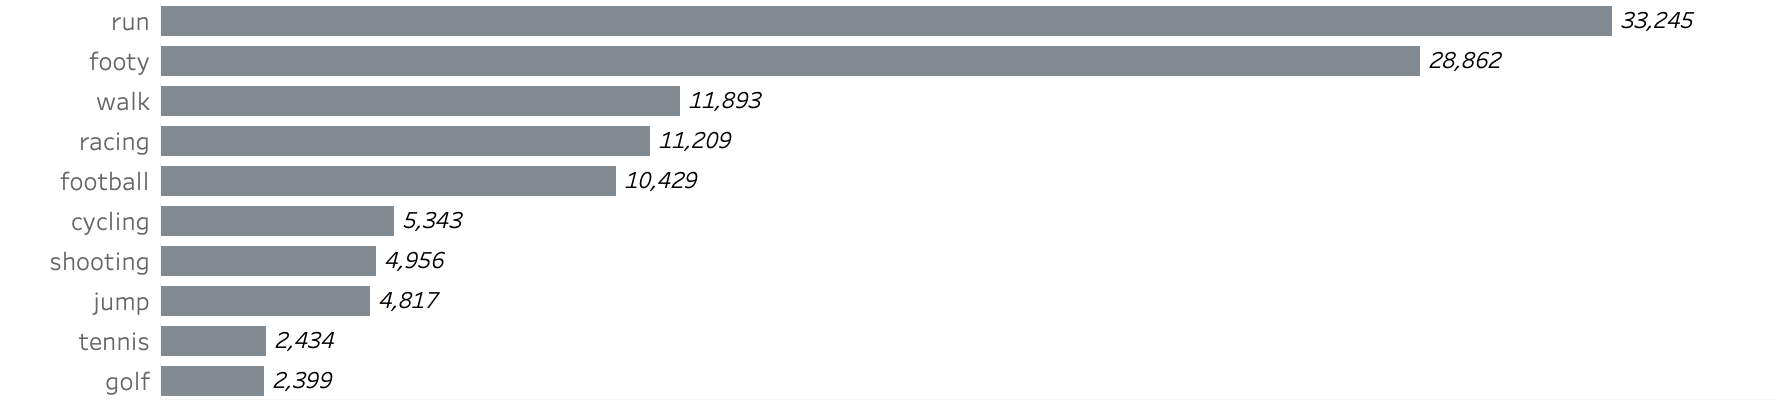
\includegraphics[width=6in]{Figures/popular sports.png}}
\caption{Top 10 Popular Sports  \label{popular sports}}
\end{figure*}

\begin{figure*}[h!]
\centerline{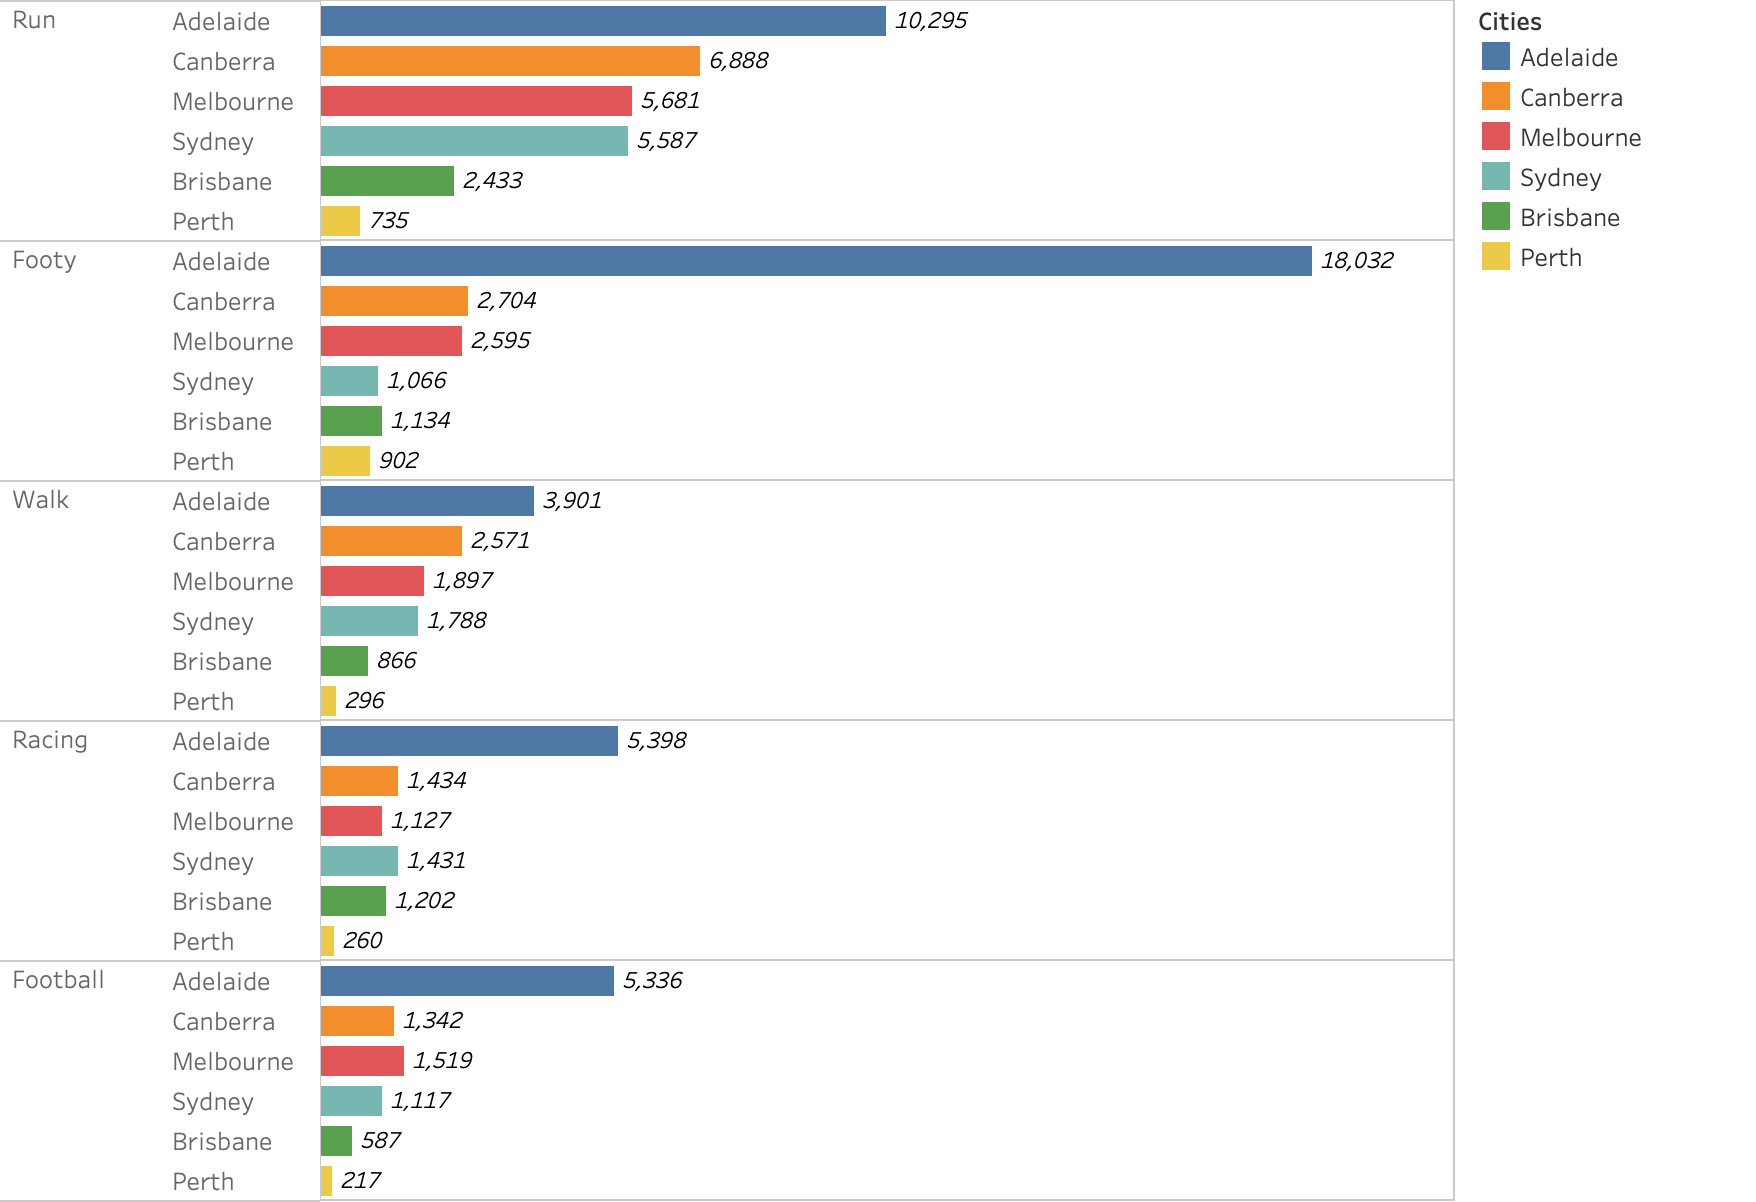
\includegraphics[width=6in]{Figures/popular sports summart.png}}
\caption{Top 5 Popular Sports of each City \label{popular sports of each city}}
\end{figure*}

Among all the sports included in our sports list, “run” is the most tweeted sport among six cities, with over 33,000 related tweets. Next comes to footy, whose number of related tweets is more than twice as "walk", "racing" and "football". "cycling", "shooting", "jump", "tennis" and "golf" whose related tweets rank from a 6 to 10, with the number under 6,000 (Figure \ref{popular sports}).

Twitter user from those six state cities shows the similar preference regarding top 5 sports ("run", "footy", "walk", "racing" and "football"), which are all outdoor activities. While users in Adelaide and Perth discussed "AFL" the most, and people in the other three cities tweeted "run" the most (Figure \ref{popular sports of each city}). 


\subsubsection{Scenario 3: Fitness enthusiasts}
Comparing to the first two scenarios, this one focuses on Twitter users. When it comes to identifying a fitness enthusiast, two factors are considered here, namely, the frequency of posting sports tweets, and the tough level of these sports. Since reducing function in CouchDB cannot be self-defined, we use MapReduce from both CouchDB and Spark to spot the top bodybuilders across the cities. 

\paragraph{CouchDB MapReduce}
MapReduce in CouchDB is used first to return the sports score of each tweet, which is the sum of difficulty points of sports mentioned in the tweet. Meanwhile, the tweet without any sports keywords is removed.  When it comes to a sport that appears in the tweet, the sports score is calculated in the map function by matching sport to related score by using Prototype. In this case, the reduce function used is \mintinline{python}{_count}, and each entry returns a username and sports score. After that, the initial result from the CouchDB view is passed to Django, which then submits the job to Spark.

\begin{lstlisting}[language=JavaScript, caption= Map Functions for Sports Score, backgroundcolor = \color{white}]
function (doc) {
//challenge scores from 75 to 1
 let scoresArr = [75, 74, ..., 2, 1]; 
 
//75 sports array
 let sportsArr=[`boxing', `hockey', ..., `jog']; 
 var score = 0;
 
//get index of challenge score of a sport
 Array.prototype.indexValue=function(arr){
  for(var i=0;i<this.length;i++){
 if(this[i]==arr){
 return i;
 }}}
 
 //get score for each tweet
 for(j = 0; j < sportsArr.length; j++){
 if (doc.val.text.includes(sportsArr[j])){
 score += scoresArr[sportsArr.indexValue(sportsArr[j])];
 }}
 
 //return username and sports score 
 if (score>0){
 emit(doc.val.user.name,score);
 }}

\end{lstlisting}

\begin{figure*}[h!]
\centerline{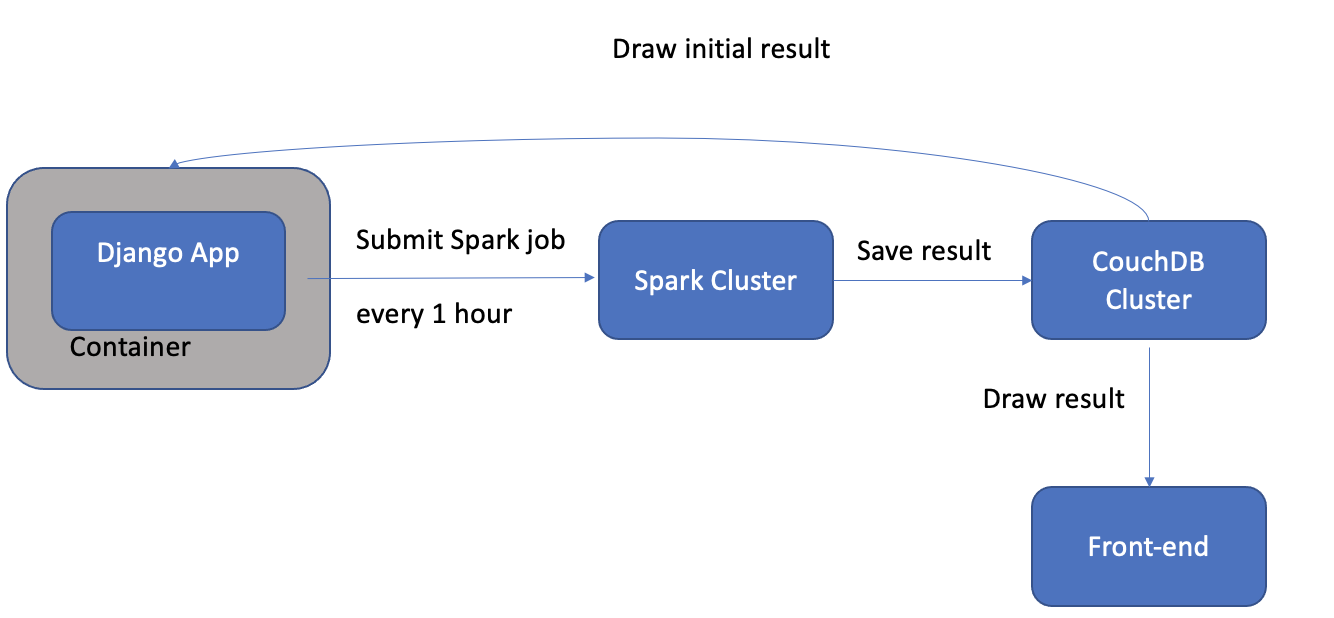
\includegraphics[width=6in]{Figures/couchdb-spark.png}}
\caption{Map Reduce in CouchDB and Spark \label{couchdb and spark}}
\end{figure*}
\paragraph{Spark RDD}
Figure \ref{couchdb and spark} illustrates that the Spark Job, where it aggregates the sports score for each user and sort them by the sport scores in a descending order. The Django application fetches the initial result from the CouchDB view and submits the job to the Spark cluster every hour. Since the top 5 sport enthusiasts does not update frequently, an update frequency of 1 hour is considered adequate for this application. As it does not require user to control, the functionalities remain at a highly usable level. 

\paragraph{Result}
It is interesting that the top 5 fitness enthusiasts' scores are very close, at around 30,000. Specifically, user "Sportageos" is the most hardworking bodybuilder, which is followed by user "Dani Abbracciavento". "Kenny Lu" comes to the third (Figure \ref{enthusiasts}).

\begin{figure}[H]
\centerline{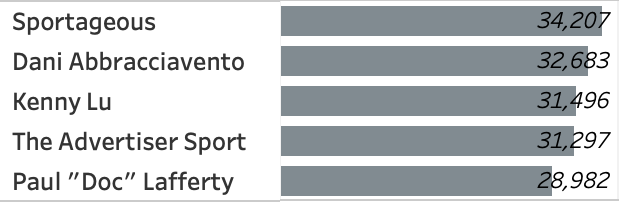
\includegraphics[width=3in]{Figures/enthusiasts.png}}
\caption{Fitness Enthusiasts \label{enthusiasts}}
\end{figure}

\subsection{Future work}
Two things were planned for future implementation.
The first one is to expand the number of cities in this application. Due to the limitation of the project timeframe and lack of data related to cities, we only analyzed and presented the data of six cities in this project. However, we designed a highly scalable backend that allows us to expand the number of cities. The procedure consists of three steps. The data and geo-locations of a new city can be firstly added into the Aurin database and the City database. After adding the data, the tweets of the city can be searched and stored by instances in MRC since the instance was designed to harvest tweets from cities in the city database. Lastly, if the tweets were stored in the Twitter database, the data can be extracted and analyzed.
 
The second future direction is implementing more scenarios and doing natural language processing. In this project, all three scenarios we analyzed mostly required keywords, so the contents of tweets were not analyzed in another aspect. However, in the future, we can provide more scenarios, for example, checking the kinds of sports that most people like or dislike. These scenarios can be presented by doing sentiment analysis on tweet contents. The analyzing process can be easily achieved since all tweet contents were already stored in the database.
